\documentclass{article}

\usepackage[utf8]{inputenc}
\usepackage[T1]{fontenc}
\usepackage[french]{babel}
\usepackage{graphicx}
\usepackage{hyperref}
\usepackage{caption}
\usepackage{amsmath}
\usepackage{amssymb}
\usepackage{amsthm}
\usepackage{minted}

\newcommand{\source}[1]{\caption*{Source: #1}}
\newcommand{\bigo}{\mathcal{O}}
\newcommand{\vertices}{\mathcal{V}}
\newcommand{\edges}{\mathcal{E}}
\newcommand{\referencetitle}[1]{\textit{#1}}
\newcommand{\noncontour}{\mathcal{NC}}
\newcommand{\R}{\mathbb{R}}
\newcommand{\rayons}{\mathcal{R}}
\newcommand{\inter}{\cap}
\newcommand{\N}{\mathbb{N}}
\newcommand{\filename}[1]{\texttt{#1}}

\setminted[python]{linenos=true}

\title{Optimisation de l'évacuation en cas d'urgence}
\author{Jean Jouve}

\begin{document}

\maketitle

\tableofcontents

\section{Étude des foules et évacuation}

L'étude du comportement des foules est un domaine important pour
améliorer la sécurité lors des évènement publics ainsi que dans
les bâtiments publics. Mais l'étude de ces foules par l'expérience
coute chère car il est nécessaire de mobiliser un grand nombre d'individus,
lors d'un simple festival de musique il peut y avoir plus de 7000 personnes.
De plus les personnes prenant pars aux expériences ne seront pas
dans les conditions réelles, ils ne seront donc pas paniqués par exemple,
l'expérience peut alors produire des résultats erronés.

La conception de bonnes expérience permettant l'étude des foules
étant difficile, l'étude se fait principalement grâce
à des simulations se basant sur des vidéos et des descriptions
d'évènements réelle ainsi que sur des résultats d'expériences
exécuté avant le développement des simulations.


\section{Objectifs}

L'objectif du TIPE de mon trinôme fut de développer ne programme
permettant d'étudier le mouvement d'une foule en cas d'évacuation
dans différentes situation. Puis d'en déduire des optimisations possibles
pour l'évacuation, particulièrement des optimisations concernant le plan
d'évacuation et la disposition des obstacles.

Le TIPE s'est découpé en deux simulations à des échelles différentes, après
le développement des simulation une étude des résultats produits par les
simulations à été faite. Une des simulations se base sur un graphe à flux
variant et  est à l'échelle d'un bâtiment, l'autre simulation se base sur
les simulations multi-agents et est à l'échelle d'une salle.

Je me suis concentré sur la modélisation du mouvement des agents dans la
simulation multi-agents, je décrirai donc seulement les
résultats de cette simulation.

\section{Simulation multi-agents}

Dans le domaine de la modélisation des foules les simulation multi-agents sont
les simulations les plus présentes. Contrairement aux modélisation se basant sur
des automates cellulaire et celles se basant sur le mouvement de particule
qui modélise le mouvement de la foule dans son ensemble, les modélisations
multi-agents modélise chaque agents individuellement le comportement de la foule
étant un résultat du comportement de chacun de ces agents.

\section{Outils utilisés}

Nous avons codé les simulations en Python car c'est le seule langage connue
par l'ensemble de notre trinôme, de plus Python viens avec un grand nombre
de modules permettant de faciliter le développement de notre simulation.

Nous avons utilisé un module de la librairie standard pour manipulé des
fichiers en JSON que nous avons utilisé comme
fichiers de configurations pour nos simulations permettant ainsi de facilité
l'étude de différentes situations.

Nous avons aussi utilisé le moteur physique en deux dimensions Pymunk,
qui est une enveloppe autour du moteur physique Chipmunk codé en C, pour
éviter de passer trop de notre temps voire tout notre temps sur la
modélisation physique des obstacles et des agents. Nous avons utilisé en
plus de Pymunk la librairie graphique Pygame pour afficher la simulation.

La structure de donnée utiliser par Pymunk pour ses calculs est une
hiérarchie de volumes englobants, une structure couramment utilisé pour la
détection de collisions dans un espace et le lancé de rayon -- j'utilise
cette disposition pour les lancé de rayons --,
c'est un arbre binaire dont chaque
nœuds est un volume qui englobe les volumes des nœuds enfants, les feuilles
de cette arbre sont les objets de l'espace (\autoref{fig:BVH}). Ainsi pour chercher les
objets intersectant un objet donnée il suffit de rechercher récursivement
dans les sous arbres dont le volume englobant racine intersecte l'objet
donnée. Pymunk utilise des rectangles aligné aux axes des abscisses et des
ordonnées couramment nommé AABB -- axis-aligned bounding box -- comme
volume englobant.
Pour avoir des recherches efficaces Pymunk équilibre l'arbre en
minimisant la surface occupé par chaque nœuds.

\begin{figure}[h]
  \centering
  \includegraphics[height=4cm]{img/BVH.pdf}
  \caption{Un exemple de BVH}
  \source{\url{https://en.wikipedia.org/wiki/Bounding_volume_hierarchy}}
  \label{fig:BVH}
\end{figure}

\section{Description d'une salle}

Les salles dans lesquelles sont étudiées le mouvement sont délimité par
une AABB représentant les murs. Des trous dans les murs représentent les
différentes sorties. (\autoref{fig:murs})

\begin{figure}[h]
  \centering
  \includegraphics[height=4cm]{img/salle.png}
  \caption{Un exemple de salle, cette salle a une sortie en bas à droite}
  \label{fig:murs}
\end{figure}

Les obstacles présent dans la salles -- rangs d'une classe, pilier, etc... --
ont d'abord était représentés par des AABB (\autoref{fig:obstacles}) car ce
sont des formes très simples
et donc ont permis de rapidement développer une modélisation correcte. Puis
ces obstacles ont était représentés par des polygones convexes quelconques
(\autoref{fig:obstacles}) pour atteindre une modélisation plus générale, la convexité
ne pose pas
de problèmes dans la généralité car tout polygones peut se décomposer en une
union de polygones convexes -- il existe une triangulation pour tout
polygones simples -- on peut donc représenté tout obstacle en accolant des
polygones convexes ensembles mais ce n'est en générale pas nécessaire.

\begin{figure}[h]
  \centering
  \includegraphics[height=4cm]{img/obstacles.png}
  \caption{Des exemples d'obstacles, une AABB à gauche et une polygone
    convexe quelconque à droite}
  \label{fig:obstacles}
\end{figure}

%Regarder une démonstration de la triangulation

\section{Description des agents}

Beaucoup de simplifications ont été faites pour les agents. Au mieux les agents
devrait être représentés par des ellipses souples car en vus de dessus les agents
ont grossièrement la forme d'ellipse et peuvent prendre plus ou moins de place
selon la pression qui leurs est appliqué -- ils plient les bras pour laisser de
la place par exemple --. Mais une ellipse est une forme qui engendre des calculs
de géométrie compliqué et lent à exécuté d'autant plus si l'ellipse est souple.
Nous avons donc choisi de représenter les agents par des disques rigides
(\autoref{fig:agent}),
cela permet d'avoir une simulation rapide sans perdre trop de réalisme, les
disques étant une assez bonne approximation d'une ellipse et la différence
de rayons entre les cas extrêmes et petite par rapport au rayon moyen.

\begin{figure}[h]
  \centering
  \includegraphics[height=4cm]{img/agent.png}
  \caption{Un agent}
  \label{fig:agent}
\end{figure}

%Essaye de trouver le rayon moyen et différence entre bras au repos et bras
%pressé contre soit

\section{Modélisation du mouvement d'un agent}

Mon objectif pour modéliser le mouvement d'un agent et de développer
un algorithmes qui trouve la direction à suivre pour atteindre
une certaine position étant donnée toutes les informations sur les
obstacles et les autres agents tout en gardant un bon réalisme.

\subsection{Mouvement en fonction du voisinage}

En situation réelle les agents ne prennent pas en compte ce qui se trouve
loin d'eux et ce qui ne se trouve pas dans leur champ de vision, le premier
algorithme place donc des points autours de l'agent à une distance de un pas
-- trois fois le rayon de l'agent --on retire ensuite dans ces points l'ensemble
des points étant inaccessibles, puis on choisi parmi les points restants le
point le plus proche de la sortie. La distance caractéristique d'un pas permet
aux points de bien prendre en compte du voisinage de l'agent tout en
évitant les obstacles avant de rentrer en collision avec ce qui est plus réaliste

Le dernier point choisi est retenue après chaque choix de direction et
l'agent continus à avancer dans cette direction jusqu'au prochain choix,
l'algorithme fait un nouveau choix lorsque le dernier point choisi se
retrouve bloqué. 

Cette algorithme n'est pas du tout efficace pour amener l'agent en dehors
de la sortie même si l'agent sort la plupart du temps, le chemin pris
est loin d'être optimale, et contrairement à ce qui était recherché
l'algorithme n'est pas du tout recherché, cela est du au manque de choix
possibles de directions qui est limité au nombre de points et est du à la
prise en compte de seulement le voisinage beaucoup trop proche qui était
forcé par le choix des points comme détection d'obstacle.

\subsection{Mouvement en fonction du champ de vision}

Pour remédier aux lacunes qu'as le choix de la direction par utilisation
de points pour détecter les obstacles, j'ai choisi de détecter les obstacles
grâce à des lancés de rayons, ceci permet de choisir parmi quasiment toutes
les directions possibles et de prendre en compte la totalité du champ de
vision de l'agent.

En plus du lancé de rayon on associe à chaque obstacle $o$ de l'espace un
ensemble d'obstacle $\noncontour(o)$ empêchant le contour de cette obstacle ,
c'est à
dire en notant $d$ la distance euclidienne, $\mathcal{O}$
l'ensemble des obstacles et $r$ le rayon de l'agent on associe à
l'obstacle $o$ l'ensemble
\[
  \left\{ o' \in \mathcal{O} \middle| d(o, o') < 2r \right\}
\]
Cette association est faite à l'aide d'une table de hachage à
adressage ouvert. -- ce sont les tables de hachages par défaut
en python --

On calcule la distance $d(o, o')$ en utilisant
le fait que cette distance est atteinte sur la frontière des obstacles,
en notant $\edges(o)$ l'ensemble des arrêtes
de l'obstacle $o$ et $\vertices(o)$ l'ensemble des sommets de
l'obstacle $o$, on a
\begin{align*}
  d(o, o') = \min\biggl\{
    &\min_{(v, v') \in \vertices(o) \times \vertices(o')} d(v, v'), \\
    &\min_{(v, e') \in \vertices(o) \times \edges(o')} d(v, e'), \\
    &\min_{(e, v') \in \edges(o) \times \vertices(o')} d(e, v')\biggr\}
\end{align*}
qui se détermine en $\bigo\left(|\vertices(o)||\vertices(o')|\right)$.

Il existe des algorithmes prenant 
$\bigo\left(\log\left(|\vertices(o)|\right)
  + \log\left(|\vertices(o')|\right)\right)$ 
de temps pour calculer cette distance car les obstacles sont
convexes \cite{YangQiMengLiWang06}, mais la complexité quadratique
n'est pas dérangeante car j'ai décidé de mettre en cache à
l'aide d'une table de hachage les distances calculés et car le nombre
de sommets par obstacles est assez faible dans la grande majorité des
salles.

Pour choisir la direction l'algorithme exécute en premier un lancé de rayon
vers la sortie et détecte ainsi si il y a un obstacle $o$ sur droite de
l'agent à la sortie, si il n'y a pas d'obstacle l'algorithme choisi
la direction de la sortie comme direction à prendre, sinon l'algorithme
recherche les rayons passant sur les bords des obstacle de $\noncontour(o)$
sans traversé aucun obstacle de $\noncontour(o)$, puis choisis le rayon
ayant la plus petite distance angulaire avec le premier rayon lancé
(\autoref{fig:choixrayons}), il fait un choix glouton.

\begin{figure}[h]
  \centering
  \includegraphics[height=4cm]{img/choisrayons.pdf}
  \caption{Le choix des rayons se fait entre $(a)$ et $(b)$, comme $\alpha > \beta$
    l'algorithme choisira $(b)$ comme rayon à suivre}
  \label{fig:choixrayons}
\end{figure}

Pour décrire l'algorithme qui recherche les rayons pour le choix glouton
on pose la fonction
\[
  f : \R \to \{1, 0\}
\]
qui à $\theta \in \R$ associe $1$ si il y a un obstacle de $\noncontour(o)$
dans cette direction et associe $0$ sinon, ainsi l'objectif de l'algorithme
est de trouver l'ensemble des angles $\theta$ tel que
$f$ change de valeur en $\theta$ c'est à dire l'ensemble
\[
  \rayons = \left\{ \theta \middle|
    f\left(\theta^-\right) \neq f\left(\theta^+\right) \right\}
\]

%L'algorithme de recherche des rayons exécute une dichotomie
%sur chaque intervalle de $\R$ où $f$ est monotone, pour trouver
%ces intervalles l'algorithme se base sur un diviser-pour-régner.
%L'algorithme prend en entrée un intervalle $I = [\alpha, \beta]$
%\begin{itemize}
%  \item si $f(\alpha) \neq f(\beta)$ on considère que $f$ est
%    monotone sur $I$-- je reviendrais plus tard sur cette considération --
%    donc on lance une dichotomie sur l'intervalle
%  \item si $f(\alpha) = f(\beta) = 1$ on 
%\end{itemize}

Pour calculer l'ensemble $\rayons$ il suffit de trouver les intervalles
sur lesquels $f$ est monotone pour pouvoir faire une dichotomie sur
chacun de ces intervalles. L'algorithme trouve les intervalles par
récurrence, il s'autorise d'omettre des rayons de $\rayons$ si
le rayon omis est sur de ne pas être le rayon le plus proche de
la sortie, il prend en entré un intervalle $I = [\alpha, \beta]$,
en notant $m = \frac{\alpha + \beta}{2}$
\begin{itemize}
  \item si $f(\alpha) = f(\beta)$ l'algorithme se relance sur $[\alpha, m]$
    et $[m, \beta]$
  \item si $f(\alpha) \neq f(\beta)$ l'algorithme considère que $f$ est
    monotone sur $I$ -- j'expliquerai cette considération -- et lance une
    dichotomie sur $I$
\end{itemize}
Ainsi l'algorithme renvois $\rayons \cap I$, donc on lance l'algorithme
avec pour entrée $I = [0, 2 \pi]$ on obtient ainsi $\R$

%Devrais je démontrer cela dans le rapport?
Lorsque l'on a $f(\alpha) \neq f(\beta)$, $f$ n'est pas forcément
monotone, on pourrait se retrouver dans le cas de
\autoref{fig:monotonie}, on a $o', o'' \in \noncontour(o)$ alors
l'agent ne peut pas passer entre $o'$ et $o''$ on peut donc changer
$f$ tel que $f(\theta) = 1$ entre $o'$ et $o''$, on peut ainsi
considérer $f$ monotone sur $[\alpha, \beta]$. Ce changement
dans $f$ n'est pas fait dans l'implémentation de l'algorithme
car je me suis rendu compte de cette propriété trop tard.

\begin{figure}[h]
  \centering
  \includegraphics[height=4cm]{img/monotnie.pdf}
  \caption{Cas particulier de la situation $f(\alpha) = f(\beta)$,
    le bleu représentant les intervalles où $f(\theta) = 0$ et le rouge
    les intervalles où $f(\theta) = 1$}
  \label{fig:monotonie}
\end{figure}

L'algorithme utilisant les lancés de rayons rend le mouvement beaucoup
plus réaliste (\autoref{fig:comparasonalgo}) et permet la sortie de la
plupart des agents mais certains agents peuvent rester bloqué 
dans certaines configurations de salle (\autoref{fig:blocage}), en fait
tout algorithme non informé, ne stockant aucune information,
utilisant un champ de vision, une fonction
$f : \R \to \N$ tel que $f(\theta)$ indique l'obstacle dans la direction
angulaire $\theta$, peut se retrouver bloqué malgré l'existence d'une
sortie.

\begin{figure}[h]
  \centering
  \includegraphics[height=4cm]{img/Trajets_MPSTAR_test_proximite.pdf}
  \includegraphics[height=4cm]{img/Trajet_MPSTAR_dicho.png}
  \caption{Trajectoire de trois agents avec l'algorithme utilisant
    le voisinage (à droite) et avoir l'algorithme utilisant le
    lancé de rayon (à gauche)}
  \label{fig:comparasonalgo}
\end{figure}

\begin{figure}[h]
  \centering
  
\includegraphics[height=4cm]{img/blocagetotale.pdf}
  \caption{Blocage de tout algorithme non informé utilisant
    un champ de vision}
  \label{fig:blocage}
\end{figure}

\subsection{Mouvement par un champ vectoriel}

On a vu qu'un agent peut se retrouver dans une situation où un
algorithme de lancé de rayon ne peut l'en sortir car l'algorithme
n'est pas informé. Pour régler ce problème j'ai supposé que
l'agent avait bonne connaissance de la salle lors de l'évacuation
il connais donc le chemin à prendre à l'avance.

Cela m'à amené à créer un champ vectoriel $\vec{C}: S \to \R^2$ sur
l'espace $S$ de la salle tel que $\vec{C}(x, y)$ indique la direction
à prendre par un agent étant à la position $(x, y)$.

Pour la première implémentation de ce champ, j'ai utilisé un
hachage de l'espace $H$ comme structure de donnée pour stocker le champ.
Un hachage de l'espace est une découpe de l'espace en cellules stocké
dans un tableau à deux dimensions qui
associe à un point $(x, y)$ de l'espace la cellule dans laquelle
le point $(x, y)$ se trouve en temps constant \cite{MacDonald09}.
On accède en temps
constant à une cellule car les indices $(i, j)$ de la cellule peuvent
être récupérés grâce à la formule
\[
  j = \left\lfloor \frac{x - H.x}{t} \right\rfloor
\]
où $H.x$ est l'abscisse du coin bas droit de l'hachage de l'espace et $t$
et la taille d'une cellule (\autoref{fig:spacehash}), la formule pour $i$
est analogue.

\begin{figure}[h]
  \centering
  \includegraphics[height=4cm]{img/spacehash.pdf}
  \caption{Un exemple d'hachage de l'espace}
  \label{fig:spacehash}
\end{figure}

Ainsi l'algorithme doit remplir chaque cellules de l'hachage de l'espace
par un vecteur indiquant la direction à prendre par un agent se trouvant
dans cette cellule. Le remplissage de l'hachage de l'espace s'est fait
par un parcours en largeur où
j'ai considérer que deux cellules sont voisines si les cellules
se touches -- deux cellules ayant des sommets se touchants se
touchent --  et si ont peut aller d'une cellule à une autre
sans rencontrer d'obstacle, pour tester cela l'algorithme fait
un lancer de rayon entre les deux cellules et indique qu'il
est possible d'aller de l'une à l'autre si aucun obstacle n'as
été touché par le lancer de rayon. Lorsque le parcours en largeur
traite une cellule il regarde toute les voisines et assigne
à chacune des cellules un vecteur dirigé vers la cellule état traité,
ainsi comme le parcours en largeur traite d'abord les cellules
proches des sortie le champ dirige progressivement les agents
vers la sortie (\autoref{fig:parcours}).

\begin{figure}[h]
  \centering
  \includegraphics[height=4cm]{img/champvectorielle.pdf}
  \caption{Un exemple de parcours, les cellule sont numéroté par l'ordre
    de traitement}
  \label{fig:parcours}
\end{figure}

On peut voire dans \autoref{fig:parcours} que le parcours en largeur ne
donne pas le plus cours chemin, cela est du à l'aspect continue de l'espace
et l'aspect discret du parcours en largeur ainsi qu'au fait que la distance
entre deux cellules n'est pas toujours $1$ mais diffère, un meilleur champ aurait
pu être obtenue en utilisant un algorithme du plus cours chemin tel l'algorithme
de Dijkstra avec des arrêtes de poids $1$ et $\sqrt{2}$ ce qui aurait permis
de mieux se rapprocher du plus cours chemin réelle au plus --
$8\%$ plus long \cite{Nash12} --, mais
un manque de temps à empêché d'implémenter cela.

\begin{figure}[h]
  \centering
  \includegraphics[height=4cm]{img/champvecteur8MPSTAR.png}
  \includegraphics[height=4cm]{img/MPSTAR.png}
  \caption{Un champ vectorielle et la salle sur lequel il a été créé}
  \label{fig:champvecteur}
\end{figure}

Le premier algorithme de champ vectorielle fait bien sortir les agents
mais le mouvement des agents n'est pas très réaliste car les agents
suivent un chemin sur un quadrillage (\autoref{fig:champvecteur}), pour
remédier à cela le second algorithme calcule un champ de gradient dérivé
d'un champ de scalaire qu'il construit. Je fait en sorte que le gradient
dépende plus de la position de l'agent que de la case où se trouve l'agent
pour atteindre un meilleur réalisme.

Cette algorithme utilise une structure de donnée que l'on nommera treillis
très similaire à celle de l'algorithme
précédent, c'est un quadrillage de l'espace qui associe à chaque croisement
du quadrillage une valeur, le treillis est tel que l'on peut récupérer
en temps constant les valeurs étant aux coins d'une case dans laquelle se
trouve un point (\autoref{fig:treillis}).

\begin{figure}[h]
  \centering
  \includegraphics[height=4cm]{img/quadrillage.pdf}
  \caption{Le treillis permet de récupérer les valeurs aux points bleus à
    partir du point}
  \label{fig:treillis}
\end{figure}

Pour remplir le treillis on procède de la même façon que pour l'algorithme
précédent, mais au lieu d'assigner des vecteurs le parcours en largeur
assigne à chaque intersection du quadrillage l'opposé de la distance
à la sortie la plus proche, ainsi le gradient donnera la direction vers
la sortie la plus proche.

Pour calculer le gradient en un point $(x, y)$ de l'espace, l'algorithme
créer un champ scalaire définis sur tout l'espace de la salle $S$ en
interpolant
les valeurs du treillis, puis l'algorithme dérive le champ scalaire en
$(x, y)$ pour avoir le gradient. Ces deux étapes sont exécutées en une seule
en dérivant directement la formule d'interpolation. L'utilisation de
l'interpolation permet de donner la dépendance recherché du gradient
à la position.

La formule d'interpolation utilisé et la formule d'interpolation
bilinéaire \cite{Wikipedia1} qui est une formule quadratique
en $x$ et $y$, elle permet d'avoir un champ continus en tous points
de l'espace et dérivable sur l'intérieur -- d'un point de vue
topologique -- des cases du quadrillage. La formule d'interpolation
bicubique \cite{Wikipedia2} permet d'avoir un champ dérivable en tout
point mais elle crée un comportement étrange chez les agents que je
n'ai pas réussi à expliquer, elle n'a donc pas été retenue.

Le champ de gradient n'as pas le manque de réalisme que le premier
algorithme a (\autoref{fig:champgradient} mais pose un problème,
les agents restent bloqués
au niveau des coins des obstacles (\autoref{fig:coingradient}).
Cela est surement du au remplissage par un parcours en largeur
qui ne donne pas la distance exacte aux sorties.

\begin{figure}[h]
  \centering
  \includegraphics[height=4cm]{img/coingradient.pdf}
  \caption{Mouvement de l'agent proche d'un coin avec l'algorithme utilisant
    un gradient}
  \label{fig:coingradient}
\end{figure}

\begin{figure}[h]
  \centering
  \includegraphics[height=4cm]{img/champgradient8precis.png}
  \includegraphics[height=4cm]{img/MPSTAR.png}
  \caption{Champ de gradient à gauche obtenue avec l'algorithme dans la
    salle à droite}
  \label{fig:champgradient}
\end{figure}

\section{Recherche d'optimisations grâce à la modélisation}

Pour rechercher les optimisations possibles, la modélisation
est utilisé avec l'algorithme utilisant les lancés de rayons,
et si il y a des obstacles dans la salles les obstacles sont
suffisamment espacé pour ne pas rentrer dans un blocage. Dans
ces conditions l'algorithme utilisant les lancés de rayons
donne un mouvement plus réaliste que l'algorithme utilisant
le champ de gradient.

La temps qu'a pris la modélisation du mouvement des agents
nous a empêché de passer beaucoup de temps sur la recherche
d'optimisation possibles, nous nous sommes donc concentré
sur la fluidification débit par le placement d'un obstacle
en face de la sortie. Cette optimisation est souvent
 mentionné dans la littérature scientifique \cite{Theos94}.

Nous avons déterminer la distribution du débit moyen de
deux salles, une vide et une autre vide avec un obstacle
devant la porte censé fluidifier le mouvement
(\autoref{fig:fluidification}). On voit clairement
que l'obstacle devant la porte réduit considérablement
le débit. Ce résultat ne veut pas dire que l'obstacle ne
fluidifie pas en situation réelle, en effet le ralentissement
que génère l'obstacle est surtout du au manque de finesse de notre
modélisation. Notre simulation ne prend pas suffisamment en compte
les interactions humaine tel que la tendance à éviter
autrui que les personnes ont (, qui est la raison du manque de
fluidification.

\begin{figure}[h]
  \centering
  \includegraphics[height=4cm]{img/salleVideObstacle.png}
  \includegraphics[height=4cm]{img/salleVide.png} \\
  \includegraphics[height=4cm]{img/ObstacleGaucheSansObstacleDroite.png}
  \caption{répartition des débit moyen d'une simulation sur 100 simulation
    pour chaque salle}
  \label{fig:fluidification}
\end{figure}

\begin{figure}[h]
  \centering
  \includegraphics[height=4cm]{img/comportement.pdf}
  \caption{Situation où un agent ralentit un autre agent lors
    de sa sortie au niveau d'un obstacle, cette situation à lieu
    car les agents n'essaient pas d'éviter les autres agents comme
    c'est le cas en situation réelle}
\end{figure}

\section{Conclusion}

Les limites de notre modélisation à permis de mettre en valeur certain
points importants dans l'implémentation d'une simulation du mouvement
de foule tel que l'intéraction entre les agents.

\appendix

\begin{thebibliography}{9}

\bibitem{YangQiMengLiWang06}
  Yang Cheng-lei,
  Qi Meng,
  Meng Xiang-xu,
  Li Xue-qing,
  Wang Jia-ye,
  \referencetitle{A new fast algorithm for computing the distance  between two disjoint convex polygons based on Voronoi diagram},
  Journal of Zhehiang University SCIENCE A,
  2006.

\bibitem{MacDonald09}
  Tristam MacDonald,
  \referencetitle{Spatial Hashing},
  \url{https://www.gamedev.net/resources/_/technical/game-programming/spatial-hashing-r2697},
  2009

\bibitem{Nash12}
  Alex Nash,
  \referencetitle{Any-Angle Path Planning},
  \url{http://idm-lab.org/bib/abstracts/papers/dissertation-nash.pdf},
  2012

\bibitem{Wikipedia1}
  Wikipedia,
  \referencetitle{Interpolation bilinéaire},
  \url{https://fr.wikipedia.org/wiki/Interpolation_bilin%C3%A9aire}

\bibitem{Wikipedia2}
  Wikipedia,
  \referencetitle{Interpolation bicubique},
  \url{https://fr.wikipedia.org/wiki/Interpolation_bicubique}

\bibitem{Flower}
  Daniel Flower,
  \referencetitle{Crowd Simulation for Emergency Response Planning}

\bibitem{Theos94}
  Constantin Theos,
  \referencetitle{Modélisation du mouvement des personnes lors de
    l'évacuation d'un bâtiment à la suite d'un sinistre},
  \url{https://tel.archives-ouvertes.fr/file/index/docid/523176/filename/1994TH_THEOS_C_NS20040.pdf},
  1994
  
\end{thebibliography}
  
\section{Listings}

\subsection{\filename{simulation.py}}
\inputminted{python}{lst/simulation.py}
\subsection{\filename{constructeur\_simulation.py}}
\inputminted{python}{lst/constructeur_simulation.py}
\subsection{\filename{espace.py}}
\inputminted{python}{lst/espace.py}
\subsection{\filename{personne.py}}
\inputminted{python}{lst/personne.py}
\subsection{\filename{test\_point\_suivre.py} (Modélisation du mouvement)}
\inputminted{python}{lst/test_point_suivre.py}
\subsection{\filename{space\_hash.py} (Hachage de l'espace et Treillis)}
\inputminted{python}{lst/space_hash.py}
\subsection{\filename{ecouteur.py}}
\inputminted{python}{lst/ecouteur.py}
\subsection{\filename{lieu\_ferme.py}}
\inputminted{python}{lst/lieu_ferme.py}
\subsection{\filename{obstacle.py}}
\inputminted{python}{lst/obstacle.py}
\subsection{\filename{representation.py}}
\inputminted{python}{lst/representation.py}
\subsection{\filename{geometrie.py}}
\inputminted{python}{lst/geometrie.py}
\subsection{\filename{base.py}}
\inputminted{python}{lst/base.py}
\subsection{\filename{fonctions\_annexes.py}}
\inputminted{python}{lst/fonctions_annexes.py}
\subsection{\filename{representation\_categories.py}}
\inputminted{python}{lst/representation_categories.py}

\end{document}
